\documentclass[a4paper,11pt]{article}
\usepackage{amsmath,amsthm,amsfonts,amssymb,amscd,amstext,vmargin,graphics,graphicx,tabularx,multicol} 
\usepackage[francais]{babel}
\usepackage[utf8]{inputenc}  
\usepackage[T1]{fontenc} 
\usepackage{pstricks-add,tikz,tkz-tab,variations}
\usepackage[autolanguage,np]{numprint} 

\setmarginsrb{1.5cm}{0.5cm}{1cm}{0.5cm}{0cm}{0cm}{0cm}{0cm} %Gauche, haut, droite, haut
\newcounter{numexo}
\newcommand{\exo}[1]{\stepcounter{numexo}\noindent{\bf Exercice~\thenumexo} : \marginpar{\hfill /#1}}
\reversemarginpar


\newcounter{enumtabi}
\newcounter{enumtaba}
\newcommand{\q}{\stepcounter{enumtabi} \theenumtabi.  }
\newcommand{\qa}{\stepcounter{enumtaba} (\alph{enumtaba}) }
\newcommand{\initq}{\setcounter{enumtabi}{0}}
\newcommand{\initqa}{\setcounter{enumtaba}{0}}

\newcommand{\be}{\begin{enumerate}}
\newcommand{\ee}{\end{enumerate}}
\newcommand{\bi}{\begin{itemize}}
\newcommand{\ei}{\end{itemize}}
\newcommand{\bp}{\begin{pspicture*}}
\newcommand{\ep}{\end{pspicture*}}
\newcommand{\bt}{\begin{tabular}}
\newcommand{\et}{\end{tabular}}
\renewcommand{\tabularxcolumn}[1]{>{\centering}m{#1}} %(colonne m{} centrée, au lieu de p par défault) 
\newcommand{\tnl}{\tabularnewline}

\newcommand{\bmul}[1]{\begin{multicols}{#1}}
\newcommand{\emul}{\end{multicols}}

\newcommand{\trait}{\noindent \rule{\linewidth}{0.2mm}}
\newcommand{\hs}[1]{\hspace{#1}}
\newcommand{\vs}[1]{\vspace{#1}}

\newcommand{\N}{\mathbb{N}}
\newcommand{\Z}{\mathbb{Z}}
\newcommand{\R}{\mathbb{R}}
\newcommand{\C}{\mathbb{C}}
\newcommand{\Dcal}{\mathcal{D}}
\newcommand{\Ccal}{\mathcal{C}}
\newcommand{\mc}{\mathcal}

\newcommand{\vect}[1]{\overrightarrow{#1}}
\newcommand{\ds}{\displaystyle}
\newcommand{\eq}{\quad \Leftrightarrow \quad}
\newcommand{\vecti}{\vec{\imath}}
\newcommand{\vectj}{\vec{\jmath}}
\newcommand{\Oij}{(O;\vec{\imath}, \vec{\jmath})}
\newcommand{\OIJ}{(O;I,J)}


\newcommand{\reponse}[1][1]{%
\multido{}{#1}{\makebox[\linewidth]{\rule[0pt]{0pt}{20pt}\dotfill}
}}

\newcommand{\titre}[5] 
% #1: titre #2: haut gauche #3: bas gauche #4: haut droite #5: bas droite
{
\noindent #2 \hfill #4 \\
#3 \hfill #5

\vspace{-1.6cm}

\begin{center}\rule{6cm}{0.5mm}\end{center}
\vspace{0.2cm}
\begin{center}{\large{\textbf{#1}}}\end{center}
\begin{center}\rule{6cm}{0.5mm}\end{center}
}



\begin{document}
\pagestyle{empty}
\titre{Interrogation: Droites parallèles et droites perpendiculaires }{Nom :}{Prénom :}{Classe}{Date}


\exo{1} 

\bmul{2}
Sur cette figure, on a tracé une droite (d) et
quatre autres droites $(d_{1})$ , $(d_{2})$ , $(d_{3})$ et $(d_{4})$.\\

Une de ces droites est \textbf{perpendiculaire} à la droite (d).
\textbf{La repasser en bleu}.\\

Une de ces droites est \textbf{parallèle} à la droite (d).
\textbf{La repasser en vert}.

\columnbreak

\psset{xunit=1.0cm,yunit=1.0cm,algebraic=true,dotstyle=o,dotsize=3pt 0,linewidth=0.8pt,arrowsize=3pt 2,arrowinset=0.25}
\begin{pspicture*}(-2.6,-0.88)(5.82,5.44)
\psplot[linewidth=1.6pt]{-2.6}{5.82}{(--14.01--1.44*x)/7.34}
\psplot{-2.6}{5.82}{(--26.27--1.44*x)/7.34}
\psplot{-2.6}{5.82}{(--4.7--1.68*x)/10.62}
\psplot{-2.6}{5.82}{(-0.52--7.34*x)/-1.44}
\psplot{-2.6}{5.82}{(--26.3-7.38*x)/0.28}
\end{pspicture*}


\emul

\exo{2} Tracer, dans chacun des cas, la droite (d') parallèle à la droite (d) et passant par le point A.\\

\includegraphics[scale=1]{ie6.eps} 


\exo{2} Tracer, dans chacun des cas, la droite (d') perpendiculaire à la droite (d) et passant par A. Coder les figures obtenues. \\


\includegraphics[scale=1]{perp.eps} 


\exo{3,5} 

\bmul{2}

\q Compléter par le symbole « $\in$ » ou «$\notin$» :\\
B ..... $(d_{2})$ D .... [BA) A .... [DB) D .... (AB)\\
\q Quel est le point d'intersection des droites
$(d_{1})$ et $(d_{2})$ ?  ........\\
\q Construire la droite $(d_{3})$ qui vérifie :\\
B $\in$ $(d_{3})$ et $(d_{3})$ $\perp$ $(d_{1})$\\
\q Construire la droite $(d_{4})$ qui vérifie :\\
C $\in$ $(d_{4})$ et $(d_{4}) \slash{}\slash{} (d_{2})$

\columnbreak
\includegraphics[scale=1]{mult.eps} 
\emul



\exo{1,5} Écrire vrai ou faux :\\

\noindent \qa Deux droites qui ne sont pas parallèles sont sécantes : ....................\\
\qa Deux droites qui ne sont pas parallèles sont perpendiculaires : ....................\\
\qa Deux droites qui sont perpendiculaires ont un point d'intersection : ....................


\end{document}
